\chapter{State of the Art} \label{chap:state_of_the_art}


\section*{Introduction}
Electricity grids, commonly referred to as “grids,” play a vital role in modern energy infrastructure. They facilitate power generation, transmission, distribution, and control. Over time, grids have evolved from localized systems to interconnected networks, adapting to meet increasing demands and technological advancements. These grids contribute significantly to economic and societal progress.

Amidst dynamic changes in the energy landscape, the emergence of the “smart grid” presents transformative possibilities. Leveraging data, automation, and connectivity, smart grids enhance energy management and promote sustainability. In this chapter, we delve into the evolution of grid systems and explore the challenges and opportunities associated with smart grid technology, shaping the future of energy.
\newpage


\section{Definition smart grid}
The Smart Grid is a comprehensive electrical network that employs cutting-edge communication technologies, computational intelligence, and cybersecurity protocols throughout the entire process of generating, transmitting, distributing, and consuming electricity. Its objective is to establish a system that is environmentally friendly, secure, dependable, adaptable, energy-efficient, and environmentally sustainable. While the ultimate vision of the Smart Grid is ambitious, its practical implementation demands careful evaluation of costs, rigorous testing, and validation. Introducing new functionalities can occur autonomously, with each necessitating justification and a reasonable return on investment. The compatibility of open systems facilitates smooth integration into the Smart Grid once the technologies have been validated \cite{gharavi2011smart}.
 The National Institute of Standards and Technology (NIST), operating within the U.S. Department of Commerce, has classified the smart grid into seven distinct domains, as illustrated in Figure \ref{fig:NIST}. A concise overview of these domains and their stakeholders is provided in Table \ref{table:domains}.\cite{gopstein2021nist}
\begin{figure}[h]
	\centering
	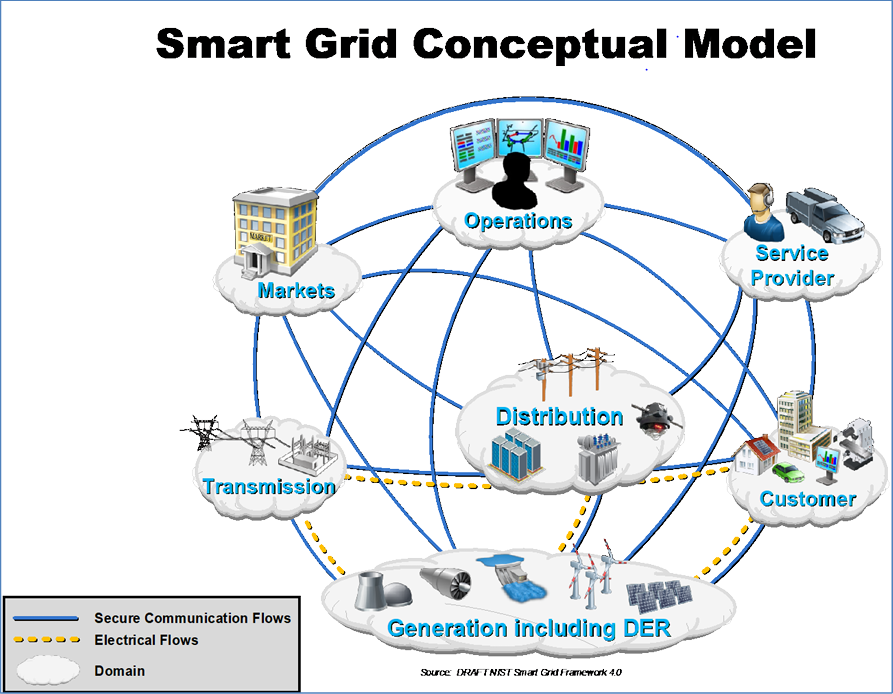
\includegraphics[width=\textwidth]{figures/nist.PNG}
	\caption{The NIST Conceptual Model for SG \cite{gopstein2021nist}}
	\label{fig:NIST}
\end{figure}
\begin{table}[h]
    \centering
 %%ffffff
    
% \begin{tabularx}{\textwidth}{|X|X|}
% \hline
% \textbf{Domain} & \textbf{Roles/Services in the Domain} \\
% \hline
% 1 Customer & The end users of electricity. May also generate, store, and manage the use of energy. Traditionally, three customer types are discussed, each with its own sub-domain: residential, commercial, and industrial. \\
% \hline
% 2 Markets & The facilitators and participants in electricity markets and other economic mechanisms used to drive action and optimize system outcomes. \\
% \hline
% 3 Service Provider & The organizations providing services to electrical customers and to utilities. \\
% \hline
% 4 Operations & The managers of the movement of electricity. \\
% \hline
% 5 Generation Including DER & The producers of electricity. May also store energy for later distribution. This domain includes traditional generation sources and distributed energy resources (DER). \\
% \hline
% 6 Transmission & The carriers of high voltage electricity over long distances. May also store and generate electricity. \\
% \hline
% 7 Distribution & The distributors of electricity to and from customers. May also store and generate electricity. \\
% \hline
% \end{tabularx}
\begin{tabular}{|p{0.15\textwidth}|p{0.8\textwidth}|}
    \hline
    \textbf{Domain} & \textbf{Roles/Services in the Domain} \\
    \hline
    1 Customer & The end users of electricity. May also generate, store, and manage the use of energy. Traditionally, three customer types are discussed, each with its own sub-domain: residential, commercial, and industrial. \\
    \hline
    2 Markets & The facilitators and participants in electricity markets and other economic mechanisms used to drive action and optimize system outcomes. \\
    \hline
    3 Service Provider & The organizations providing services to electrical customers and to utilities. \\
    \hline
    4 Operations & The managers of the movement of electricity. \\
    \hline
    5 Generation Including DER & The producers of electricity. May also store energy for later distribution. This domain includes traditional generation sources and distributed energy resources (DER). \\
    \hline
    6 Transmission & The carriers of high voltage electricity over long distances. May also store and generate electricity. \\
    \hline
    7 Distribution & The distributors of electricity to and from customers. May also store and generate electricity. \\
    \hline
    \end{tabular}
    \caption{Domains and their associated roles/services \cite{gopstein2021nist}}
    \label{table:domains}
\end{table}
\section{Smart grid attributes}
Many smart grid advocates cite some or all of its following attributes as representative of its promise:
\firmlist
\begin{itemize}


\item \textbf{  Efficiency:} Capable of meeting growing consumer demand without the need for additional infrastructure.

\item \textbf{  Flexibility: }Able to accept energy from various sources, including solar and wind, with the same ease as traditional fuels like coal and natural gas. It can integrate new technologies, such as energy storage, as they become commercially viable.

\item \textbf{  Empowering: }Facilitating real-time communication between consumers and utility providers, allowing consumers to adjust their energy usage based on factors like price and environmental concerns.

\item \textbf{  Opportunistic:} Creating new markets and opportunities by leveraging plug-and-play innovations whenever suitable.

\item\textbf{   Focus on Quality:} Able to deliver reliable power without disruptions, ensuring the smooth operation of digital technologies crucial to our economy.

\item \textbf{  Resilience:} Increasingly resistant to cyber attacks and natural disasters through decentralization and the implementation of smart grid security measures.

\item \textbf{  Environmental Sustainability:} Contributing to the mitigation of climate change and offering a viable path towards reducing the environmental impact of electricity generation. \cite{el2014smart}
\end{itemize}


\section{Differences between Traditional grid and Smart grid }
Table \ref{tab:comparison} offers a thorough comparison of the conventional power grid with the smart grid. In contrast to the traditional grid where customers play a passive role, the smart grid actively engages them through bi-directional communication technologies. For instance, rooftop photovoltaic solar panels produce electricity during the day, enabling customers to sell surplus energy back to the grid. At night, these panels continue to power home appliances as usual. Moreover, the smart grid incorporates innovative technologies like distributed generation, electric vehicle charging and discharging, and Flexible Alternating Current Transmission Systems (FACTS) to improve energy distribution and management.\cite{zhang2014smart}
\begin{table}[h]
  
	\caption{Comparison between conventional grid and smart grid \cite{miller2008understanding}}
    

	\begin{tabular}{|p{3cm}|p{6cm}|p{6cm}|}
	\hline
	Aspects & Conventional Grid & Smart Grid \\
	\hline
	Interaction between Grid and Customers & Customers passively accept service from grid & Customers participation on the grid action \\
	\hline
	Renewable Energy Integration & Having trouble with renewable penetration & Integration with renewable resources enhancement \\
	\hline
	Options for Customers & No choice for customer, monopoly market & With digital market trading, PHEV, introduce bids and competition, more choice for customer \\
	\hline
	Options on Power Quality (PQ) & No choice on power quality, no price plan options for consumers & Power quality levels for different consumers \\
	\hline
	System Operation & Ageing power assets, no efficient operation & Assets operating optimization, less power loss \\
	\hline
	Protection & Only rely on protection devices, fault detect manually & Have capability of self-healing, less damage affected by fault \\
	\hline
	Reliability and Security & Susceptible to physical and cyber attack & More reliable for national security and human safety \\
	\hline
	\end{tabular}

	\label{tab:comparison}
\end{table}


\section{Components of the Smart Grid }  

\subsection{Smart Meters}
The interplay between smart meters and smart grids is depicted in Figure \ref{fig:SmartMeter}. From the perspective of the smart grid, the applications primarily revolve around leveraging smart meters to facilitate the coordination of various electrical devices, thereby achieving a dependable power system. Simultaneously, these applications strive to enhance the performance and efficiency of smart metering. These objectives align with the defining characteristics of smart grids, which drive the advancement of smart meter technologies.\cite{chen2023control}
\begin{figure}[h]
	\centering
	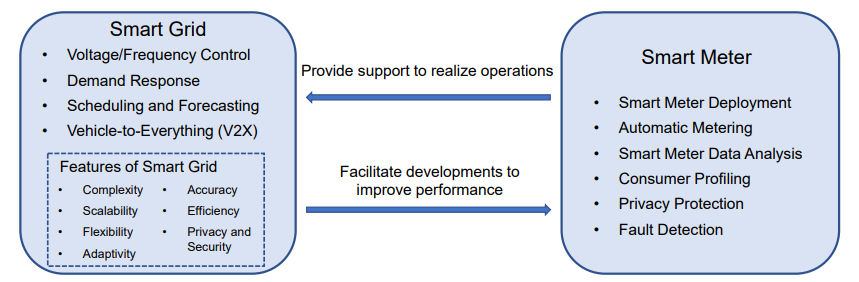
\includegraphics[width=\textwidth]{figures/SmartMeter.PNG}
	\caption{Applications from smart grid and smart meter perspectives. \cite{chen2023control}}
	\label{fig:SmartMeter}
\end{figure}
\subsection{Advanced Distribution Management Systems }
An ADMS is a software platform designed to support the comprehensive suite of tasks related to managing and optimizing the distribution of electricity. It encompasses functions that automate outage recovery and enhance the effectiveness of the distribution grid. These functions being developed for electric utilities include fault location, isolation, and restoration; optimization of voltage and reactive power; energy conservation through voltage reduction; management of peak demand; as well as support for microgrids and electric vehicles \cite{avazov2016advanced}.

% \firmlist
% \begin{itemize}


% \item \textbf{ Optimizing Power Flow:} ADMS dynamically adjusts power distribution to ensure efficient energy transfer across the grid.

% \item \textbf{  Real-Time Monitoring: }They keep a vigilant eye on the grid, promptly detecting issues like outages.

% \item \textbf{  Rerouting Electricity: }When problems arise, ADMS reroutes electricity to minimize disruptions.

% \end{itemize}
\subsection{Communication Infrastructure}
\subsection{Smart Appliances and Devices}
\subsection{Renewable Energy Integration}

% \section{Benefits of Smart Grid}  
\subsection{Increased Efficiency}
\subsection{Improved Reliability}
\subsection{Sustainability and Environmental Benefits}
\subsection{Cost Savings}
\subsection{Consumer Empowerment}
\section{Challenges of smart grid }  
\subsection{Cybersecurity}
Without a shred of doubt, cybersecurity stands out as one of the foremost and intricate challenges confronting IoT devices. Sensors, devices, and networks connected to the internet are persistent targets for various online threats like probing, espionage, ransomware, theft, and potential destruction. Considering that an IoT-driven smart grid can encompass potentially millions of interconnected nodes spread across extensive geographic regions, it emerges as the most susceptible to substantial cyber assaults. Consequently, a cyber-attack on such a system would have devastating consequences, leading to significant financial losses and potentially bringing entire countries to a standstill. The diagram in Figure \ref{fig:attacks} illustrates the number of articles reviewed per year of publication and smart grids impacted by cyber-attacks. Hence, security stands as a major hurdle in both the deployment and operation of IoT-based smart grid networks.\cite{kimani2019cyber}.
\begin{figure}[h]
	\centering
	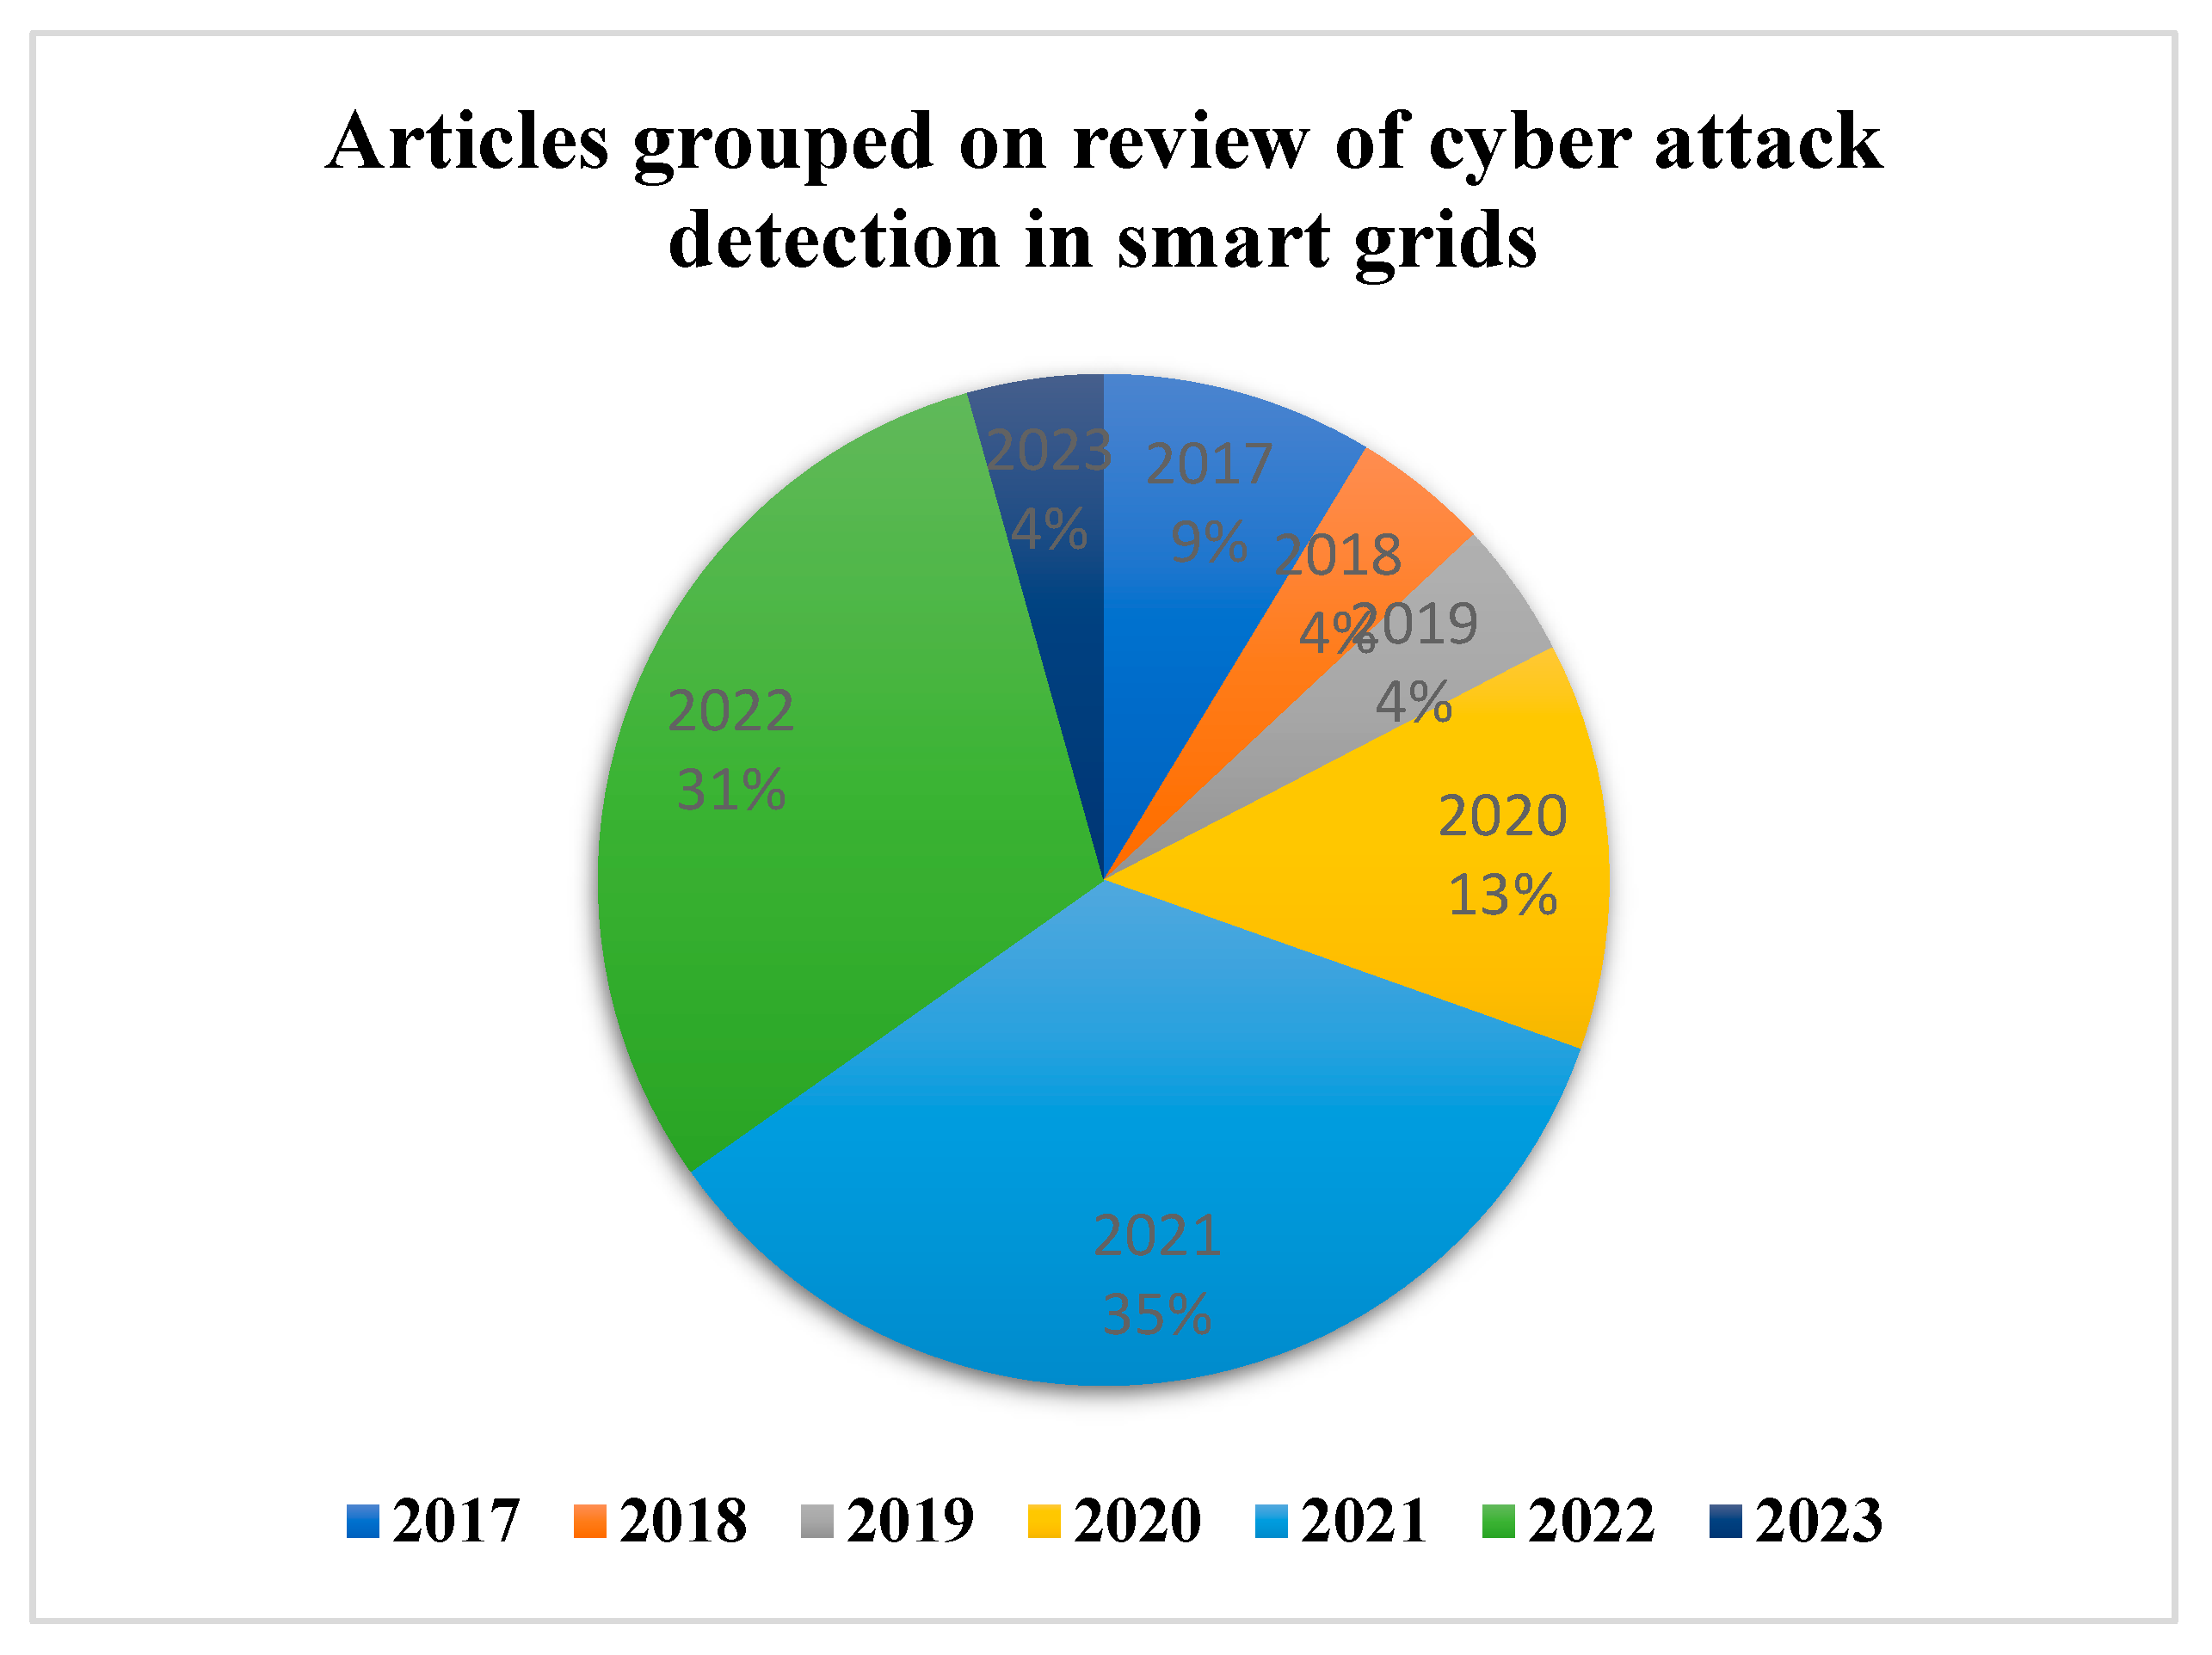
\includegraphics[width=12cm]{figures/attack.png}
	\caption{Estimate: cyber attacks will increase exponentially \cite{mdpi-link}}
	\label{fig:attacks}
\end{figure}
\newpage
\subsection{Data privacy}
Privacy is a critical concern within smart grid networks, prompting significant questions about the creation of policies regarding user data privacy. These questions revolve around several key points: Who owns the customer data? How is access to and usage of customer data regulated? What measures exist to protect the privacy and security of customer data from potential risks like surveillance or illicit activities? Is it permissible to sell or transfer customer data, and under what circumstances and for whose benefit? In areas with retail choice, are measures necessary to ensure that competing electricity providers have equal access to customer data compared to the incumbent utility?

In competitive environments among electricity providers, access to users' electricity usage patterns and behavioral information holds significant importance. Providers or their representatives may use this data to develop business strategies and create tailored packages or offers. In an open market scenario, some data may be disclosed after offers are made public, providing a level playing field for information access. However, if privacy is compromised beforehand, with specific user data available to only certain parties, these electricity providers could potentially gain unfair advantages. Therefore, effective privacy policies are essential to prevent the exploitation of unfair means in shaping business strategies.

The integration of Information and Communication Technologies (ICTs) into smart grid operations introduces various privacy concerns. Depending on how a consumer uses and recharges electricity \cite{zeadally2013towards}.

\subsection{Cost of Implementation:}

Estimating Smart Grid costs poses challenges due to several factors. Integrating digital technology into Smart Grids introduces complexities, as the failure rates and life expectancy of embedded assets differ from traditional grid technologies. For instance, a substation transformer designed for 40 years may be coupled with information technology lasting 10, 15, or 20 years, necessitating careful cost considerations for upgrades. Additionally, the rapid obsolescence of digital tech complicates estimates, as advancing communications and computational capabilities may render Smart Grid components obsolete before their intended lifespan ends. 

Moreover, the evolution of Smart Grid technologies is expected to outpace conventional tech in terms of cost reduction and advancements. However, uncertainties persist, particularly with new and unproven Smart Grid technologies. If their performance is subpar or degrades unexpectedly, it could jeopardize the entire technology's viability and business plan. As Smart Grid component costs decrease rapidly due to maturation and increased production, estimating replacement costs becomes challenging\cite{smartgrid}.
\begin{figure}[h]
	\centering
	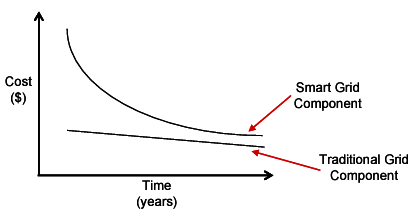
\includegraphics[width=12cm]{figures/cost.PNG}
	\caption{Grid Component Costs \cite{smartgrid}}
	\label{fig:costs}
\end{figure}
\subsection{Regulatory Frameworks}
\subsection{Public Awareness and Education}
\section{The Future of Smart Grids }  
\subsection{Distributed Generation}
\subsection{Energy Storage}
\newpage
\section*{Conclusion}
The smart grid revolution is not a destination, but a continuous journey towards a more efficient, reliable, and sustainable energy future. While challenges exist, the potential benefits of the smart grid are undeniable. By embracing innovation, fostering collaboration, and empowering consumers, we can unlock the full potential of this transformative technology.

A smarter grid paves the way for a future where clean energy sources like solar and wind power are seamlessly integrated, homes and businesses actively participate in energy management, and power outages become a rarity. It's a future where we have a more secure and sustainable energy infrastructure for generations to come.

Let's continue exploring the exciting world of smart grids and work together to build a brighter energy future for all.